\section{Logical Design}

\subsection{Transformation of the Entity-Relationship Schema}


\subsubsection{Redundancy Analysis}
The schema does not contain any cycle of entities.

\subsubsection{Choice of Principal Identifiers}
The main identifiers comply with the selection criteria.

\subsection{Analysis of Database Load}
If we consider the \textit{Research Team}'s attribute ``Number of Members" as derived, we can have the following two operations that involve that redundant attribute:
\begin{itemize}
    \item[\textbf{O1}] Store Research Personnel data and the Research Team he/she belongs to.
    \item[\textbf{O2}] Print data about a Research Team with the Number of Members it includes.
\end{itemize}
In Table~\ref{table:4}, the two operations are described. Both \textbf{O1} and \textbf{O2} are online since the Research Personnel data need to be
stored right after the Research Personnel register and join a Research Team, and Research Team data are retrieved on the fly.
\begin{longtable}[width=\textwidth]{|p{.25\columnwidth}|p{.30\columnwidth} |p{.15\columnwidth}|p{.15\columnwidth}|}
\hline
\textbf{Operation} & \textbf{Description} & \textbf{Frequency} & \textbf{Type} \\
\hline
\textbf{O1}: Store Research Personnel data & Store data about a Research Personnel including the Research Team she/he belongs to &50/week &Online \\
\hline
\textbf{O2}: Print data about a Research Team & Print data about a Research Team, including the Number of Members &10/week &Online \\
\hline

\caption{Operations description and frequency.}
\label{table:4}
\end{longtable}

In Table~\ref{table:5}, we report the access/volume data related to \textbf{O1} with redundancy. The \textit{Research Team} entity has a read access to get the current value for the Number of Members attribute and a write access to update this value.

\begin{longtable}{|p{.20\columnwidth}|p{.20\columnwidth}|p{.10\columnwidth}|p{.10\columnwidth}|p{.20\columnwidth}|}
\hline
\multicolumn{5}{|c|}{\textbf{Operation O1: 50/week}}\\\hline
\textbf{Concept} & \textbf{Construct} & \textbf{Access} & \textbf{Type} & \textbf{Average Access} \\
\hline
Research Personnel & Entity & 1 & W & $1 \times 50 \times 2 = 100$\\
Works-in & Relationship & 1 & W & $1 \times 50 \times 2 = 100$\\
Research Team & Entity & 1 & R & $1 \times 50 \times 1 = 50$\\
Research Team & Entity & 1 & W & $1 \times 50 \times 2 = 100$\\
\hline
\multicolumn{4}{|c|}{\textbf{Total access}} & 350\\
\hline
\caption{Access/volume Table for Operation 1 with redundancy.}
\label{table:5}
\end{longtable}

In Table~\ref{table:6}, we report the access/volume data related to \textbf{O2} with redundancy. The presence of redundancy
allows us to perform one access to the Research Team entity to get all the required information.

\begin{longtable}{|p{.20\columnwidth}|p{.20\columnwidth}|p{.10\columnwidth}|p{.10\columnwidth}|p{.20\columnwidth}|}
\hline
\multicolumn{5}{|c|}{\textbf{Operation O2: 10/week}}\\\hline
\textbf{Concept} & \textbf{Construct} & \textbf{Access} & \textbf{Type} & \textbf{Average Access} \\
\hline
Research Team & Entity & 1 & R & $1 \times 10 \times 1 = 10$\\
\hline
\multicolumn{4}{|c|}{\textbf{Total access}} & 10\\
\hline
\caption{Access/volume Table for Operation 2 with redundancy.}
\label{table:6}
\end{longtable}

In Table~\ref{table:7}, we report the access/volume data related to \textbf{O1} without redundancy. In this case, we have to
consider the insertion of a new instance in Research Personnel and the insertion of a new instance in Work-in to store the Research Team that the Research Personnel instance has joined.

\begin{longtable}{|p{.20\columnwidth}|p{.20\columnwidth}|p{.10\columnwidth}|p{.10\columnwidth}|p{.20\columnwidth}|}
\hline
\multicolumn{5}{|c|}{\textbf{Operation O1: 50/week}}\\\hline
\textbf{Concept} & \textbf{Construct} & \textbf{Access} & \textbf{Type} & \textbf{Average Access} \\
\hline
Research Personnel & Entity & 1 & W & $1 \times 50 \times 2 = 100$\\
Works-in & Relationship & 1 & W & $1 \times 50 \times 2 = 100$\\
\hline
\multicolumn{4}{|c|}{\textbf{Total access}} & 200\\
\hline
\caption{Access/volume Table for Operation 1 without redundancy.}
\label{table:7}
\end{longtable}

In Table~\ref{table:8}, we report the access/volume data related to \textbf{O2} without redundancy. We considered 25 Research Personnel members on average for each Research Team.

\begin{longtable}{|p{.20\columnwidth}|p{.20\columnwidth}|p{.10\columnwidth}|p{.10\columnwidth}|p{.20\columnwidth}|}
\hline
\multicolumn{5}{|c|}{\textbf{Operation O2: 10/week}}\\\hline
\textbf{Concept} & \textbf{Construct} & \textbf{Access} & \textbf{Type} & \textbf{Average Access} \\
\hline
Research Team & Entity & 1 & R & $1 \times 10 \times 1 = 10$\\
Works-in & Relationship & 25 & R & $25 \times 10 \times 1 = 250$\\
\hline
\multicolumn{4}{|c|}{\textbf{Total access}} & 260\\
\hline
\caption{Access/volume Table for Operation 2 without redundancy.}
\label{table:8}
\end{longtable}

In Table~\ref{table:9}, we report the final access count with and without redundancy. According to the obtained results, maintaining the derived attribute \textit{Number of Members} improves the load analysis.

\begin{longtable}{|p{.3\columnwidth}|p{.3\columnwidth}|p{.3\columnwidth}|}
\hline
\multicolumn{3}{|c|}{\textbf{Comparison}}\\\hline
\textbf{Operation} & \textbf{With Redundancy} & \textbf{Without Redundancy}\\
\hline
\textbf{O1} &350 &200\\
\textbf{O2} &10 &260\\
\hline
Total Accesses/week  & \textbf{360} &460\\
\hline
\caption{Comparison of the number of accesses for each operation.}
\label{table:9}
\end{longtable}

Similarly, it is possible to consider another example for a better understanding of the analysis of the database load. The \textit{Group}'s attribute ``Number of Samples" can be seen as derived and involved in the following two operations:
\begin{itemize}
    \item[\textbf{O3}] Store Sample data and the Group it belongs to.
    \item[\textbf{O4}] Print data about a Group of samples, with the Number of Samples included.
\end{itemize}
These two operations are reported in Table~\ref{table:10}. Both \textbf{O3} and \textbf{O4} are online since the Sample data need to be stored immediately after being registered and assigned to a Group whose data are retrieved in real-time.
\begin{longtable}[width=\textwidth]{|p{.25\columnwidth}|p{.30\columnwidth} |p{.15\columnwidth}|p{.15\columnwidth}|}
\hline
\textbf{Operation} & \textbf{Description} & \textbf{Frequency} & \textbf{Type} \\
\hline
\textbf{O3}: Store Sample data & Store data about a Sample including the Group it belongs to &500/day &Online \\
\hline
\textbf{O4}: Print Group data & Print data about a Group, including the Number of Samples that compose it &100/day &Online \\
\hline

\caption{Operations description and frequency.}
\label{table:10}
\end{longtable}

In Table~\ref{table:11}, the access/volume data related to \textbf{O3} with redundancy are reported. For this operation, the \textit{Group} entity has both a Read-type access to get the current value for the Number of Samples attribute and a Write-type access to update this value. The \textit{Sample} entity and the \textit{Belongs} relationship have both a Write-type access because of the Sample and Group data storage.

\begin{longtable}{|p{.20\columnwidth}|p{.20\columnwidth}|p{.10\columnwidth}|p{.10\columnwidth}|p{.20\columnwidth}|}
\hline
\multicolumn{5}{|c|}{\textbf{Operation O3: 500/day}}\\\hline
\textbf{Concept} & \textbf{Construct} & \textbf{Access} & \textbf{Type} & \textbf{Average Access} \\
\hline
Sample & Entity & 1 & W & $1 \times 500 \times 2 = 1000$\\
Belongs & Relationship & 1 & W & $1 \times 500 \times 2 = 1000$\\
Group & Entity & 1 & R & $1 \times 500 \times 1 = 500$\\
Group & Entity & 1 & W & $1 \times 500 \times 2 = 1000$\\
\hline
\multicolumn{4}{|c|}{\textbf{Total access}} & 3500\\
\hline
\caption{Access/volume Table for Operation 3 with redundancy.}
\label{table:11}
\end{longtable}

In Table~\ref{table:12}, the access/volume data related to \textbf{O4} with redundancy are reported. The presence of the redundant attribute allows only one access to the Group entity to get all the required information.

\begin{longtable}{|p{.20\columnwidth}|p{.20\columnwidth}|p{.10\columnwidth}|p{.10\columnwidth}|p{.20\columnwidth}|}
\hline
\multicolumn{5}{|c|}{\textbf{Operation O4: 100/day}}\\\hline
\textbf{Concept} & \textbf{Construct} & \textbf{Access} & \textbf{Type} & \textbf{Average Access} \\
\hline
Group & Entity & 1 & R & $1 \times 100 \times 1 = 100$\\
\hline
\multicolumn{4}{|c|}{\textbf{Total access}} & 100\\
\hline
\caption{Access/volume Table for Operation 4 with redundancy.}
\label{table:12}
\end{longtable}

In Table~\ref{table:13}, the access/volume data related to \textbf{O3} without redundancy are reported. In this case, the insertion of a new instance in the Group entity and of a new instance in the Belongs relationship have to be considered, to store properly the Group to which the Sample has been assigned.

\begin{longtable}{|p{.20\columnwidth}|p{.20\columnwidth}|p{.10\columnwidth}|p{.10\columnwidth}|p{.20\columnwidth}|}
\hline
\multicolumn{5}{|c|}{\textbf{Operation O3: 500/day}}\\\hline
\textbf{Concept} & \textbf{Construct} & \textbf{Access} & \textbf{Type} & \textbf{Average Access} \\
\hline
Sample & Entity & 1 & W & $1 \times 500 \times 2 = 1000$\\
Belongs & Relationship & 1 & W & $1 \times 500 \times 2 = 1000$\\
\hline
\multicolumn{4}{|c|}{\textbf{Total access}} & 2000\\
\hline
\caption{Access/volume Table for Operation 3 without redundancy.}
\label{table:13}
\end{longtable}

In Table~\ref{table:14}, the access/volume data related to \textbf{O4} without redundancy are reported. The average number of Samples for each Group considered to perform the analysis is 50, corresponding to the number of accesses for the Belongs relationship.

\begin{longtable}{|p{.20\columnwidth}|p{.20\columnwidth}|p{.10\columnwidth}|p{.10\columnwidth}|p{.20\columnwidth}|}
\hline
\multicolumn{5}{|c|}{\textbf{Operation O4: 100/day}}\\\hline
\textbf{Concept} & \textbf{Construct} & \textbf{Access} & \textbf{Type} & \textbf{Average Access} \\
\hline
Group & Entity & 1 & R & $1 \times 100 \times 1 = 100$\\
Belongs & Relationship & 50 & R & $50 \times 100 \times 1 = 5000$\\
\hline
\multicolumn{4}{|c|}{\textbf{Total access}} & 5100\\
\hline
\caption{Access/volume Table for Operation 4 without redundancy.}
\label{table:14}
\end{longtable}

In Table~\ref{table:15}, the final access counts with and without redundancy are reported. The obtained results suggest maintaining the derived attribute \textit{Number of Samples}, because it significantly improves the load analysis, especially as the assumed value of the attribute increases.

\begin{longtable}{|p{.3\columnwidth}|p{.3\columnwidth}|p{.3\columnwidth}|}
\hline
\multicolumn{3}{|c|}{\textbf{Comparison}}\\\hline
\textbf{Operation} & \textbf{With Redundancy} & \textbf{Without Redundancy}\\
\hline
\textbf{O3} &3500 &2000\\
\textbf{O4} &100 &5100\\
\hline
Total Accesses/day  & \textbf{3600} &7100\\
\hline
\caption{Comparison of the number of accesses for each operation.}
\label{table:15}
\end{longtable}

\newpage

\subsection{Relational Schema}
Figure 2 shows the relational schema.
\begin{center}
\begin{figure}[htp!]
    \centering
    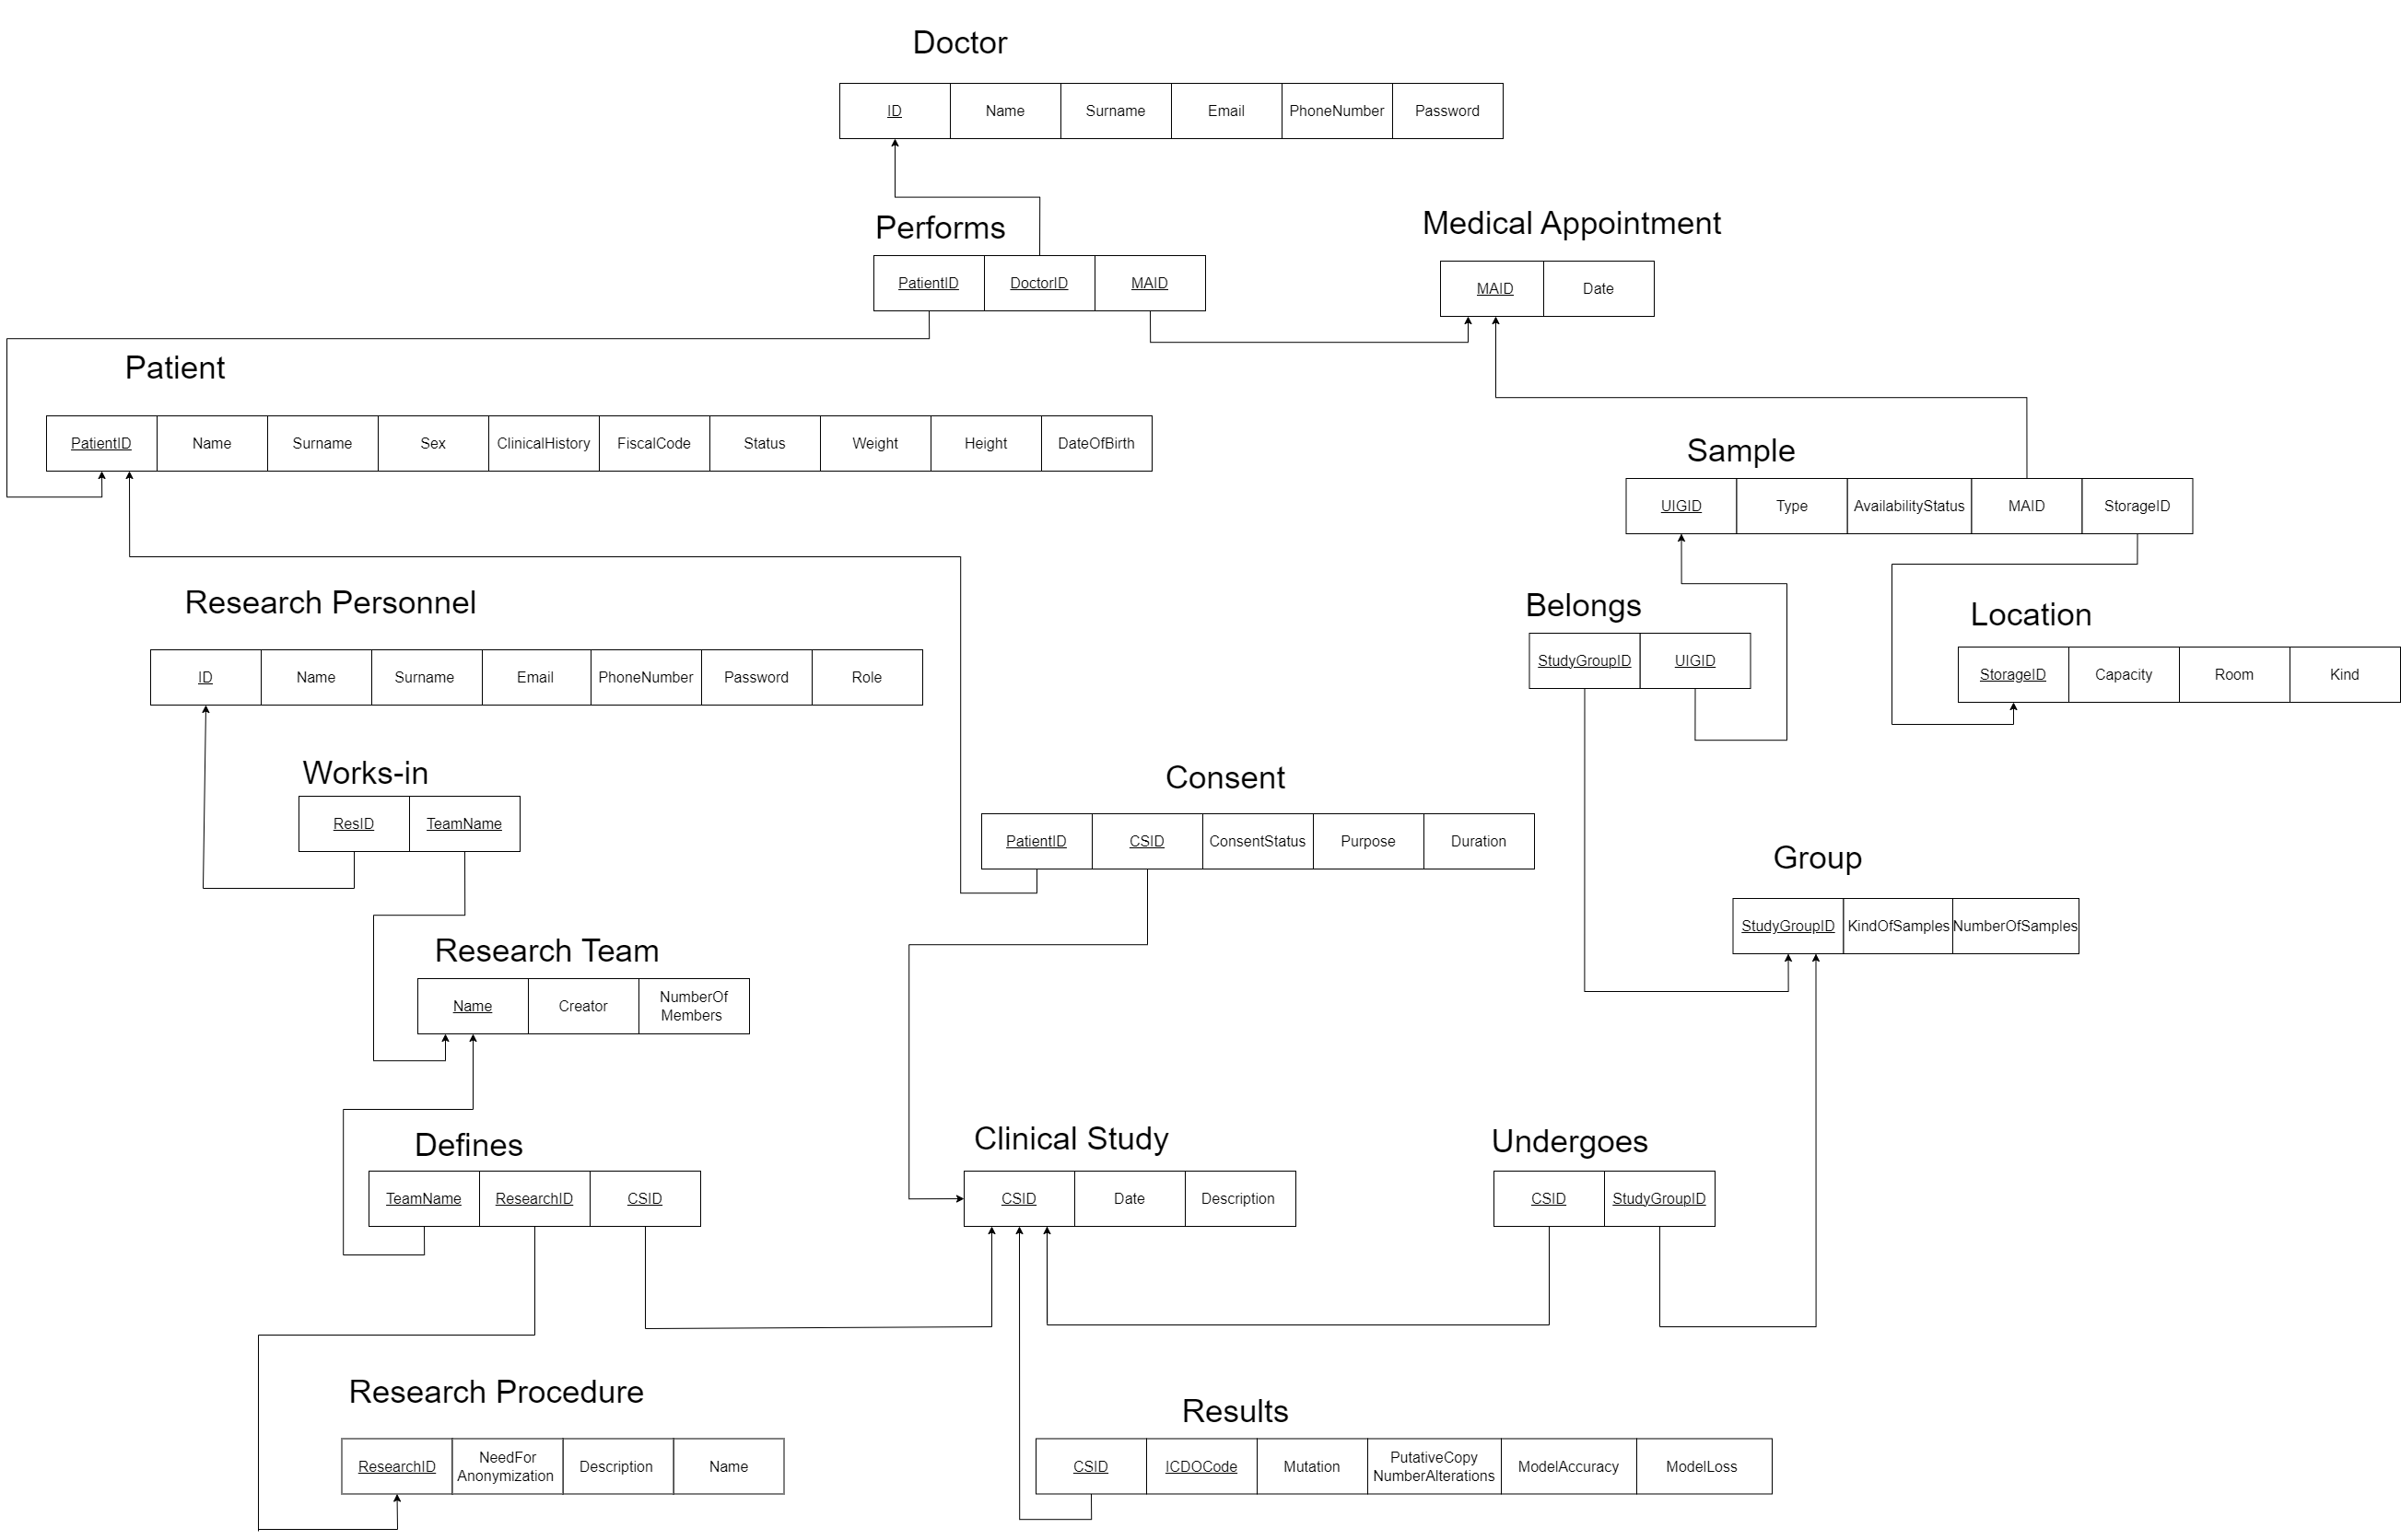
\includegraphics[width=\textwidth]{src/schemas/RelationalSchema.png}
    \caption{Relational Schema.}
\end{figure}
\end{center}

\newpage
\subsection{Data Dictionary}

\begin{longtable}{|p{.20\columnwidth}|p{.15\columnwidth} |p{.30\columnwidth}|p{.10\columnwidth}|p{.20\columnwidth} |} 
\hline
\textbf{Relation} & \textbf{Attribute} & \textbf{Description} & \textbf{Domain} & \textbf{Constraints} \\\hline

\multirow{2}{*}{Belongs}
% Sample / Group
	& UIGID
		& Unique identifier of the Sample. 
		& Serial
		& Foreign key to Sample, Not NULL, primary key with Study Group ID
\\\cline{2-5}
	& StudyGroupID
		& Unique identifier of the Group to which the Sample belongs.
		& Text
		& Foreign key to Group, Not NULL, primary key with UIGID
\\\hline

\multirow{3}{*}{Clinical Study} 
&CSID 
    &Unique identifier of the Clinical Study. 
    &Text  
    &Primary key
\\\cline{2-5}
&Date 
    &When the Clinical Study has been performed.
    &Date range 
    &Not NULL
\\\cline{2-5}
&Description 
    &The description of the study’s objectives and main features. 
    &Text 
    &
\\\hline

\multirow{3}{*}{Consent} 
&ConsentStatus 
    &It identifies whether the Patient gave or not the Consent for her/his data to be processed.
    &Boolean
    &Not NULL
\\\cline{2-5}
&Purpose 
    &Why the Patient is asked for Consent.
    &Text
    &Not NULL
\\\cline{2-5}
&Duration 
    &Period of time for which the Consent is maintained.
    &Date range
    &Not NULL
    \\\cline{2-5}
&PatientID 
    &ID of the patient giving the consent.
    &Serial
    &Foreign Key to Patient, Not NULL, primary key with CSID
\\\cline{2-5}
&CSID 
    &ID of the clinical study requiring the consent.
    &Text
    &Foreign Key to Clinical Study, Not NULL, primary key with PatientID
\\\hline

\multirow{3}{*}{Defines}
% Research Team / Clinical Study / Research Procedure
	& TeamName 
		& Unique identifier of the Research Team, carrying out the Clinical Study. 
		& Text
		& Foreign key to Research Team, Not NULL, primary key with CSID and Research ID
\\\cline{2-5}
	& CSID 
		& Unique identifier of the Clinical Study. 
		& Text
		& Foreign key to Clinical Study, Not NULL, primary key with Name and Research ID
\\\cline{2-5}
	& ResearchID 
		& Unique identifier of the Research Procedure chosen for the Clinical Study. 
		& Text
		& Foreign key to Research Procedure, Not NULL, primary key with Name and CSID
\\\hline

\multirow{6}{*}{Doctor} 
&ID 
    &Unique identifier of the Doctor.
    &Text
    &Primary key
\\\cline{2-5}
&Name
    &The name of the Doctor
    &Text
    &Not NULL
\\\cline{2-5}
&Surname 
    &The surname of the Doctor.
    &Text
    &Not NULL
\\\cline{2-5}
&Email 
    &The e-mail address of the Doctor.
    &Text
    &Not NULL
\\\cline{2-5}
&Password 
    &The log-in hashed password of the Doctor.
    &Text
    &Not NULL
\\\cline{2-5}
&PhoneNumber 
    &The phone number of the Doctor.
    &Text
    &Not NULL
\\\hline

\multirow{2}{*}{Group} 
&StudyGroupID 
    &Unique identifier of the Group to which the Sample belongs.
    &Text
    &Primary key
\\\cline{2-5}
&KindOfSamples 
    &The type of Sample collected.
    &Text
    &Not NULL
\\\hline

\multirow{4}{*}{Location} 
&StorageID
    &Unique identifier of the Location of the Sample.
    &Text
    &Primary key
\\\cline{2-5}
&Room
    &The room where the Sample is stored.
    &Text
    &Not NULL
\\\cline{2-5}
&Capacity 
    &The number of Sample each Location can contain.
    &Integer
    &Not NULL
\\\cline{2-5}
&Kind 
    &The type of sample storage Location.
    &Text
    &Not NULL
\\\hline

\multirow{2}{*}{Medical Appointment} 
&MAID 
    &Unique identifier of the Medical Appointment.
    &Text
    &Primary key
\\\cline{2-5}
&Date
    &The date when the Medical Appointment has been performed.
    &Date range
    &Not NULL
\\\hline

\multirow{10}{*}{Patient} 
&PatientID 
    &Unique identifier of the Patient.
    &Serial
    &Primary key
\\\cline{2-5}
&Name 
    &The name of the Patient.
    &Text
    &Not NULL
\\\cline{2-5}
&Surname 
    &The surname of the Patient.
    &Text
    &Not NULL
\\\cline{2-5}
&DateOfBirth 
    &The date of birth of the Patient.
    &Date range
    &Not NULL
\\\cline{2-5}
&FiscalCode
    &The fiscal code of the Patient.
    &Text
    &
\\\cline{2-5}
&Height 
    &The height of the Patient.
    &Integer
    &Not NULL
\\\cline{2-5}
&Weight 
    &The weight of the Patient.
    &Integer
    &Not NULL
\\\cline{2-5}
&Sex 
    &The sex of the Patient.
    &Text
    &Not NULL
\\\cline{2-5}
&Status 
    &Identifies if the Patient is sick or healthy.
    &Boolean
    &Not NULL
\\\cline{2-5}
&ClinicalHistory 
    &Description of the Patient's clinical history.
    &Text
    &
\\\cline{2-5}
&ConsentStatus 
    &It identifies whether the Patient gave or not the Consent for her/his data to be processed.
    &Boolean
    &Foreign key to Consent
\\\hline
\newpage
\hline
\multirow{3}{*}{Performs}
% Doctor / Medical Appointment / Patient
	& DoctorID 
		& Unique identifier of the Doctor performing the Medical Appointment. 
		& Text
		& Foreign key to Doctor, Not NULL, primary key with MAID and PatientID
\\\cline{2-5}
	& MAID 	
		& Unique identifier of the Medical Appointment. 
		& Text
		& Foreign key to Medical Appointment, Not NULL, primary key with ID and Patient ID
\\\cline{2-5}
    & PatientID 
    		& Unique identifier of the Patient. 
    		& Serial
    		& Foreign key to Patient, Not NULL, primary key with DoctorID and MAID
\\\hline

\multirow{7}{*}{Research Personnel} 
&ID 
    &Unique identifier of the Research Personnel member.
    &Text
    &Primary key
\\\cline{2-5}
&Name 
    &The name of the Research Personnel member.
    &Text
    &Not NULL
\\\cline{2-5}
&Surname
    &The surname of the Research Personnel member.
    &Text
    &Not NULL
\\\cline{2-5}
&Email
    &The e-mail of the Research Personnel member.
    &Text
    &Not NULL
\\\cline{2-5}
&Password 
    &The log-in hashed password of the Research Personnel member.
    &Text
    &Not NULL
\\\cline{2-5}
&PhoneNumber
    &The phone number of the Research Personnel member.
    &Text
    &Not NULL
\\\cline{2-5}
&Role
    &Identifies whether the Research Personnel member is a Clinical Engineer or a Data Scientist
    &Boolean
    & Not NULL
\\\hline

\multirow{4}{*}{Research Procedure} 
&ResearchID 
    &Unique identifier of the Research Procedure.
    &Text
    &Primary key
\\\cline{2-5}
&Name
    &Identifies the adopted procedure.
    &Text
    &Not NULL
\\\cline{2-5}
&Description 
    &Description of objectives and main features of the adopted Research Procedure
    &Text
    &Not NULL
\\\cline{2-5}
&NeedFor Anonymization 
    &Identifies whether the adopted Research Procedure has to be anonymized or not.
    &Boolean
    &Not NULL
\\\hline

\multirow{2}{*}{Research Team} 
&Name 
    &Unique identifier of the Research Team.
    &Text
    &Primary key
\\\cline{2-5}
&NumberOf Members 
    &The number of members of the Research Team.
    &Integer
    &Not NULL
\\\hline

\newpage
\hline
\multirow{5}{*}{Results} 
&ICDOCode 
    &Unique identifier of the Results.
    &Text
    &Primary key
\\\cline{2-5}
&Mutation 
    &Number of mutation of the Sample.
    &Integer
    &Not NULL
\\\cline{2-5}
&PutativeCopy NumberAlterations
    &Measures the genomics instability.
    &Float
    &Not NULL
\\\cline{2-5}
&ModelAccuracy 
    &Value of the accuracy metric that describes the performance of the statistical model used.
    &Float
    &
\\\cline{2-5}
&ModelLoss 
    &Value of the loss metric of the statistical model used.
    &Float
    &
\\\cline{2-5}
& CSID 
    & Unique identifier of the Clinical Study.
    & Text 
    & Foreign key to Clinical Study, Not NULL, primary key with ICD-O Code.
\\\hline

\multirow{3}{*}{Sample} 
&UIGID 
    &Unique identifier of the Sample.
    &Serial
    &Primary key
\\\cline{2-5}
&Type
    &The type of the Sample.
    &Text
    &Not NULL
\\\cline{2-5}
&AvailabilityStatus 
    &Identifies whether the Sample is available or not.
    &Boolean
    &Not NULL
\\\cline{2-5}
&MAID 
    &Unique identifier of the Medical Appointment. 
    &Text
    &Foreign key to Medical Appointment
\\\cline{2-5}
&StorageID 
    &Unique identifier of the Location of the Sample.
    &Int
    &Foreign key to Location
\\\hline

\multirow{2}{*}{Undergoes}
% Group / Clinical study 
	& StudyGroupID
		& Unique identifier of the Group which undergoes the Clinical Study.
		& Text
		& Foreign key to Group, Not NULL, primary key with CSID
\\\cline{2-5}
	& CSID 
		& Unique identifier of the Clinical Study. 
		& Text
		& Foreign key to Clinical Study, Not NULL, primary key with Study Group ID
\\\hline

\multirow{2}{*}{Works-in}
% Research Personnel / Research Team
	& ResID 
		& Unique identifier of the Research Personnel member who works in the Research Team. 
		& Text
		& Foreign key to Research Personnel, Not NULL, primary key with TeamName
\\\cline{2-5}
	& TeamName 
		& Unique identifier of the Research Team. 
		& Text
		& Foreign key to Research Team, Not NULL, primary key with ResID
\\\hline

\end{longtable}

\subsection{External Constraints}
\begin{itemize}
    \item Each research team must comprise at least one clinical engineer and one data scientist from the research personnel: this means that it is important to check the value assumed by the Role attribute for each Research Personnel tuple to be sure that at least a tuple of the Works-in relation is related to a research personnel member with role ``Clinical Engineer", and at least one with role ``Data Scientist".
    Moreover, the attribute 'Number of Members' of the 'Research Team' entity must be updated each time a new member gets added or removed from the group: this update must be done whenever a new tuple, which ResID must match the ID of the correspondent research personnel member, is added to the Works-in relation.
    \item A medical appointment can produce a sample only before having the consent form from the patient: this means that it is necessary to check in the Consent relation if the patient has given her/his consent for the processing of her/his data (ConsentStatus attribute, which must also have the same value for Patient and Clinical Study).
    \item The attribute 'Number of Samples' of the 'Group' entity must be updated each time a new sample gets added or removed from the group: in this case, it is necessary to check the Belongs relation to see when a new sample is added to a group or if a sample is no longer available (Availability Status attribute for Sample).
    \item A clinical study can be carried out insofar as it stays between the boundaries provided by the CEUR and not for other scopes: in this case, to conduct a clinical study and for each tuple of the Consent relation that assumes the value “given” for its ConsentStatus attribute, it is necessary to check the Purpose attribute and verify whether what is reported matches what is established by the CEUR.
\end{itemize}